\documentclass[aspectratio=169]{beamer}

\usetheme{default}
\usecolortheme{dove}

\setbeamertemplate{navigation symbols}{}
\setbeamertemplate{footline}{%
  \hfill{\large\insertframenumber\,/\,\inserttotalframenumber}\hspace{0.8em}\vspace{0.5em}%
}

\definecolor{popblue}{RGB}{52, 101, 164}
\definecolor{sampred}{RGB}{204, 0, 0}
\definecolor{paramgreen}{RGB}{0, 140, 70}
\definecolor{warnred}{RGB}{180, 40, 40}
\definecolor{orange1}{RGB}{220, 120, 0}
\definecolor{violet1}{RGB}{120, 50, 160}
\definecolor{lightbg}{RGB}{245, 245, 250}

\setbeamercolor{frametitle}{fg=popblue}
\setbeamercolor{title}{fg=popblue}

\usepackage{pgfplots}
\usepackage{tikz}
\usetikzlibrary{shapes, arrows.meta, positioning, calc, decorations.pathreplacing, patterns}
\pgfplotsset{compat=1.18}
\usepackage{amsmath, amssymb}
\usepackage{pifont}
\usepackage{colortbl}
\usepackage{fontenc}

\title{Lecture 12: Regression Inference}
\subtitle{From Fitting Lines to Testing Coefficients}
\date{}

\begin{document}

% ============================================================
\begin{frame}
\titlepage
\end{frame}

% ============================================================
\begin{frame}
\frametitle{Previously, on Lectures 10 \& 11\ldots}

\begin{center}
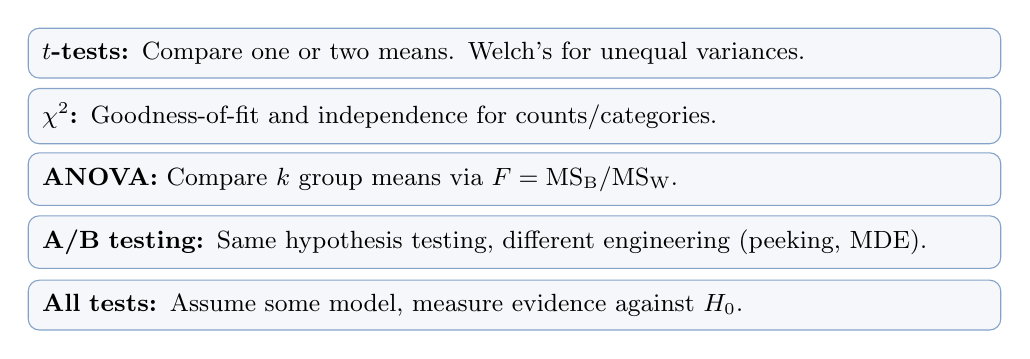
\begin{tikzpicture}[
  sbox/.style={draw=popblue!60, fill=popblue!5, rounded corners=4pt, text width=12cm, minimum height=0.5cm, align=left, inner sep=5pt, font=\small}
]
  \node[sbox] at (0, 2.0) {\textbf{$t$-tests:} Compare one or two means. Welch's for unequal variances.};
  \node[sbox] at (0, 1.2) {\textbf{$\chi^2$:} Goodness-of-fit and independence for counts/categories.};
  \node[sbox] at (0, 0.4) {\textbf{ANOVA:} Compare $k$ group means via $F = \text{MS}_\text{B}/\text{MS}_\text{W}$.};
  \node[sbox] at (0, -0.4) {\textbf{A/B testing:} Same hypothesis testing, different engineering (peeking, MDE).};
  \node[sbox] at (0, -1.2) {\textbf{All tests:} Assume some model, measure evidence against $H_0$.};
\end{tikzpicture}
\end{center}

\vspace{0.3cm}
\begin{center}
{\large\textbf{Today:}} The most widely used model in statistics: \textbf{linear regression}.\\
Not just fitting a line --- testing \textit{which predictors matter} and \textit{how much}.
\end{center}
\end{frame}

% ============================================================
% PART I: THE LINEAR MODEL
% ============================================================
\section{The Linear Model}

\begin{frame}
\begin{center}
  \vspace{1.5cm}
  {\Huge\bfseries\textcolor{popblue}{Part I: The Linear Model}}

  \vspace{0.8cm}
  {\large From the math module to the statistical framework}
\end{center}
\end{frame}

\begin{frame}
\frametitle{Quick Recall: OLS Regression}

\begin{center}
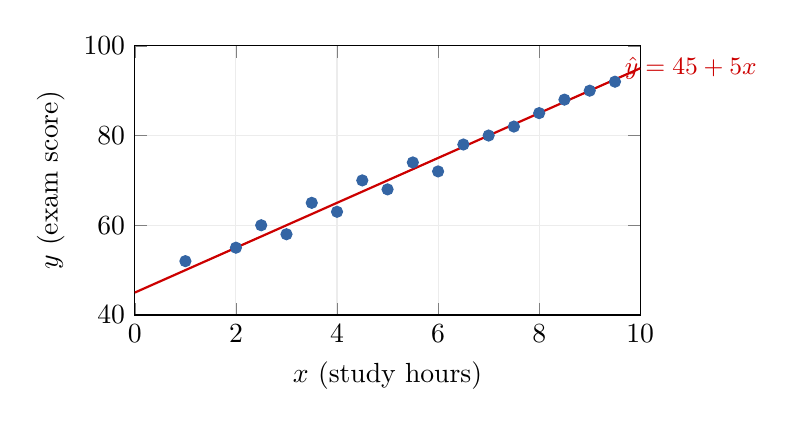
\begin{tikzpicture}
  \begin{axis}[
    width=8cm, height=5cm,
    xlabel={$x$ (study hours)},
    ylabel={$y$ (exam score)},
    xmin=0, xmax=10, ymin=40, ymax=100,
    grid=major, grid style={gray!15},
    clip=false
  ]
    % Scatter points
    \addplot[only marks, mark=*, mark size=2pt, popblue] coordinates {
      (1,52) (2,55) (2.5,60) (3,58) (3.5,65) (4,63) (4.5,70)
      (5,68) (5.5,74) (6,72) (6.5,78) (7,80) (7.5,82) (8,85)
      (8.5,88) (9,90) (9.5,92)
    };
    % Regression line
    \addplot[sampred, thick, domain=0:10] {45 + 5*x};
    \node[font=\small, sampred, right] at (axis cs:9.5, 95) {$\hat{y} = 45 + 5x$};
  \end{axis}
\end{tikzpicture}
\end{center}

\begin{center}
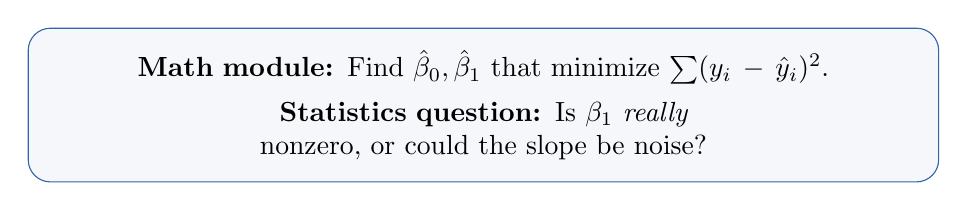
\begin{tikzpicture}
  \node[draw=popblue, fill=popblue!5, rounded corners=8pt, text width=11cm, align=center, inner sep=8pt] {
    \textbf{Math module:} Find $\hat{\beta}_0, \hat{\beta}_1$ that minimize $\sum(y_i - \hat{y}_i)^2$.\\[4pt]
    \textbf{Statistics question:} Is $\beta_1$ \textit{really} nonzero, or could the slope be noise?
  };
\end{tikzpicture}
\end{center}
\end{frame}

\begin{frame}
\frametitle{The Statistical Model}

\begin{center}
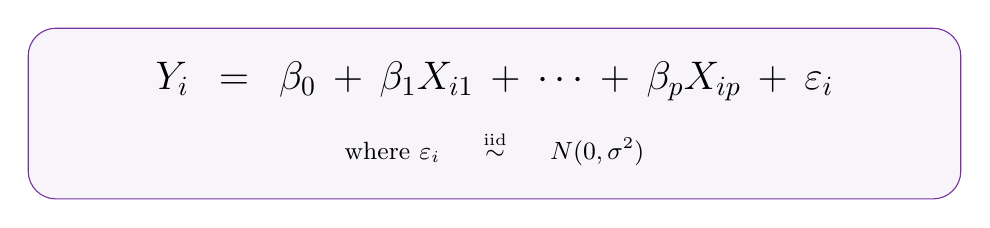
\begin{tikzpicture}
  \node[draw=violet1, fill=violet1!5, rounded corners=10pt, text width=11cm, align=center, inner sep=12pt] {
    {\Large $Y_i = \beta_0 + \beta_1 X_{i1} + \cdots + \beta_p X_{ip} + \varepsilon_i$}\\[10pt]
    \small where $\varepsilon_i \stackrel{\text{iid}}{\sim} N(0, \sigma^2)$
  };
\end{tikzpicture}
\end{center}

\vspace{0.2cm}
\begin{center}
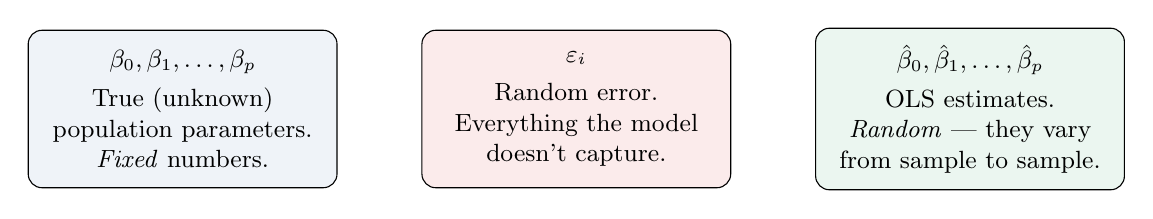
\begin{tikzpicture}[
  cbox/.style={draw, rounded corners=5pt, text width=3.5cm, align=center, inner sep=6pt, font=\small, minimum height=2cm}
]
  \node[cbox, fill=popblue!8] at (-5, 0) {
    {\bfseries $\beta_0, \beta_1, \ldots, \beta_p$}\\[3pt]
    True (unknown)\\
    population parameters.\\
    \textit{Fixed} numbers.
  };
  \node[cbox, fill=sampred!8] at (0, 0) {
    {\bfseries $\varepsilon_i$}\\[3pt]
    Random error.\\
    Everything the model\\
    doesn't capture.
  };
  \node[cbox, fill=paramgreen!8] at (5, 0) {
    {\bfseries $\hat{\beta}_0, \hat{\beta}_1, \ldots, \hat{\beta}_p$}\\[3pt]
    OLS estimates.\\
    \textit{Random} --- they vary\\
    from sample to sample.
  };
\end{tikzpicture}
\end{center}

\vspace{0.15cm}
\begin{center}
\small \textbf{Key shift:} $\hat{\beta}$ has a \textit{sampling distribution}, just like $\bar{X}$ from L7.
\end{center}
\end{frame}

\begin{frame}
\frametitle{Assumptions of the Linear Model}

\begin{center}
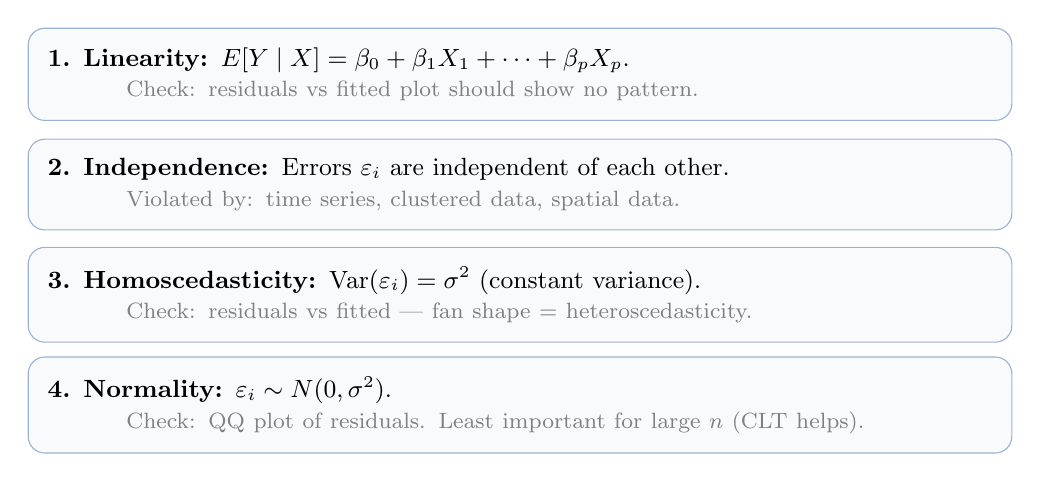
\begin{tikzpicture}[
  abox/.style={draw=popblue!50, fill=popblue!3, rounded corners=6pt, text width=12cm, align=left, inner sep=7pt, font=\small}
]
  \node[abox] at (0, 2.8) {
    \textbf{1. Linearity:} $E[Y \mid X] = \beta_0 + \beta_1 X_1 + \cdots + \beta_p X_p$.\\
    \hspace{1cm}\textcolor{black!50}{\footnotesize Check: residuals vs fitted plot should show no pattern.}
  };
  \node[abox] at (0, 1.4) {
    \textbf{2. Independence:} Errors $\varepsilon_i$ are independent of each other.\\
    \hspace{1cm}\textcolor{black!50}{\footnotesize Violated by: time series, clustered data, spatial data.}
  };
  \node[abox] at (0, 0.0) {
    \textbf{3. Homoscedasticity:} $\text{Var}(\varepsilon_i) = \sigma^2$ (constant variance).\\
    \hspace{1cm}\textcolor{black!50}{\footnotesize Check: residuals vs fitted --- fan shape = heteroscedasticity.}
  };
  \node[abox] at (0, -1.4) {
    \textbf{4. Normality:} $\varepsilon_i \sim N(0, \sigma^2)$.\\
    \hspace{1cm}\textcolor{black!50}{\footnotesize Check: QQ plot of residuals. Least important for large $n$ (CLT helps).}
  };
\end{tikzpicture}
\end{center}

\vspace{0.15cm}
\begin{center}
\small Mnemonic: \textbf{LINE} --- Linearity, Independence, Normality, Equal variance.
\end{center}
\end{frame}

% ============================================================
% PART II: INFERENCE FOR COEFFICIENTS
% ============================================================
\section{Inference for Coefficients}

\begin{frame}
\begin{center}
  \vspace{1.5cm}
  {\Huge\bfseries\textcolor{popblue}{Part II: Inference for Coefficients}}

  \vspace{0.8cm}
  {\large SE, $t$-tests, $p$-values, and CIs for each $\beta_j$}
\end{center}
\end{frame}

\begin{frame}
\frametitle{The Sampling Distribution of $\hat{\beta}$}
\framesubtitle{OLS estimates are random variables with known distributions}

\begin{center}
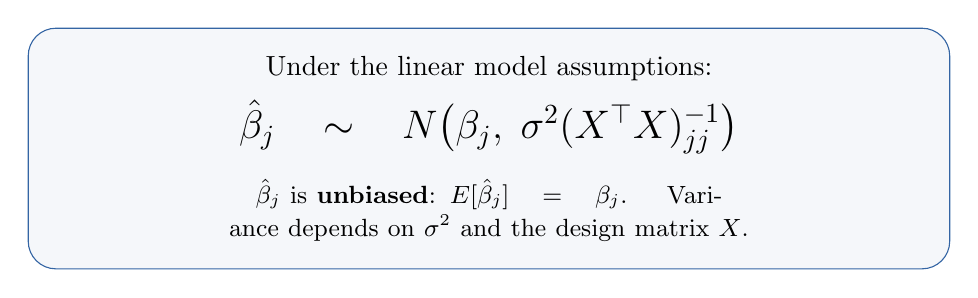
\begin{tikzpicture}
  \node[draw=popblue, fill=popblue!5, rounded corners=10pt, text width=11cm, align=center, inner sep=10pt] {
    Under the linear model assumptions:\\[6pt]
    {\Large $\hat{\beta}_j \sim N\!\left(\beta_j,\; \sigma^2 (X^\top X)^{-1}_{jj}\right)$}\\[8pt]
    \small $\hat{\beta}_j$ is \textbf{unbiased}: $E[\hat{\beta}_j] = \beta_j$. \quad
    Variance depends on $\sigma^2$ and the design matrix $X$.
  };
\end{tikzpicture}
\end{center}

\pause
\vspace{0.2cm}
\begin{center}
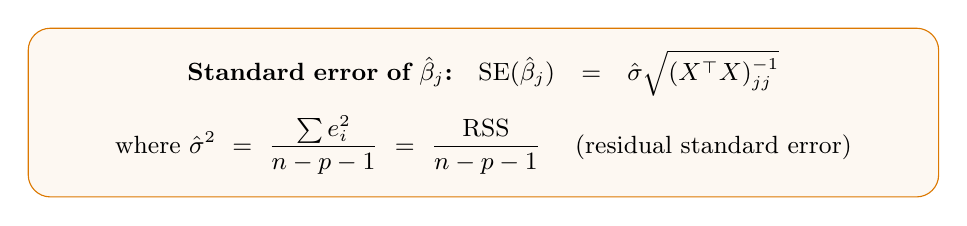
\begin{tikzpicture}
  \node[draw=orange1, fill=orange1!5, rounded corners=8pt, text width=11cm, align=center, inner sep=8pt, font=\small] {
    \textbf{Standard error of $\hat{\beta}_j$:}\quad
    $\text{SE}(\hat{\beta}_j) = \hat{\sigma}\sqrt{(X^\top X)^{-1}_{jj}}$\\[6pt]
    where $\hat{\sigma}^2 = \dfrac{\sum e_i^2}{n - p - 1} = \dfrac{\text{RSS}}{n - p - 1}$ \quad (residual standard error)
  };
\end{tikzpicture}
\end{center}

\vspace{0.15cm}
\begin{center}
\small This is just SE $=$ (estimated SD) $/$ (effective $\sqrt{n}$), same idea as L7.
\end{center}
\end{frame}

\begin{frame}
\frametitle{Simple Linear Regression: SE Formula}
\framesubtitle{For $Y = \beta_0 + \beta_1 X + \varepsilon$, the formulas simplify}

\begin{center}

\begin{tikzpicture}
  \node[draw=popblue, fill=popblue!5, rounded corners=10pt, text width=11cm, align=center, inner sep=10pt] {
    {\large $\text{SE}(\hat{\beta}_1) = \dfrac{\hat{\sigma}}{\sqrt{\sum_{i=1}^{n}(X_i - \bar{X})^2}}$}\\[10pt]
    \small $\hat{\sigma} = \sqrt{\text{RSS}/(n-2)}$
  };
\end{tikzpicture}
\end{center}

\vspace{0.2cm}
\begin{center}
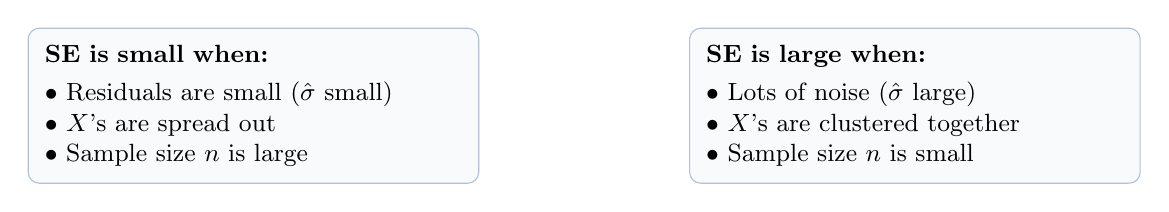
\begin{tikzpicture}[
  fbox/.style={draw=popblue!40, fill=popblue!3, rounded corners=4pt, text width=5.3cm, align=left, inner sep=6pt, font=\small}
]
  \node[fbox] at (-4.2, 0) {
    \textbf{SE is small when:}\\[3pt]
    $\bullet$ Residuals are small ($\hat{\sigma}$ small)\\
    $\bullet$ $X$'s are spread out\\
    $\bullet$ Sample size $n$ is large
  };
  \node[fbox] at (4.2, 0) {
    \textbf{SE is large when:}\\[3pt]
    $\bullet$ Lots of noise ($\hat{\sigma}$ large)\\
    $\bullet$ $X$'s are clustered together\\
    $\bullet$ Sample size $n$ is small
  };
\end{tikzpicture}
\end{center}

\vspace{0.15cm}
\begin{center}
\small Intuition: a slope is hard to estimate when $X$ doesn't vary much (imagine all points at $X = 5$).
\end{center}
\end{frame}

\begin{frame}
\frametitle{$t$-Test for a Single Coefficient}

\begin{center}
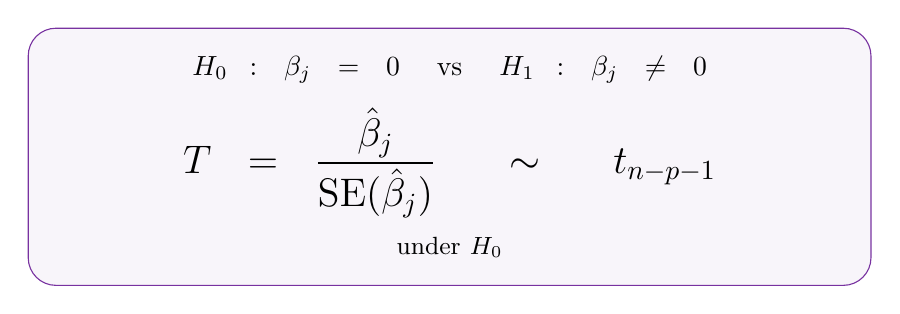
\begin{tikzpicture}
  \node[draw=violet1, fill=violet1!5, rounded corners=10pt, text width=10cm, align=center, inner sep=10pt] {
    $H_0\!: \beta_j = 0$ \quad vs \quad $H_1\!: \beta_j \neq 0$\\[8pt]
    {\Large $T = \dfrac{\hat{\beta}_j}{\text{SE}(\hat{\beta}_j)} \;\sim\; t_{n-p-1}$}\\[6pt]
    \small under $H_0$
  };
\end{tikzpicture}
\end{center}

\vspace{0.2cm}
\begin{center}
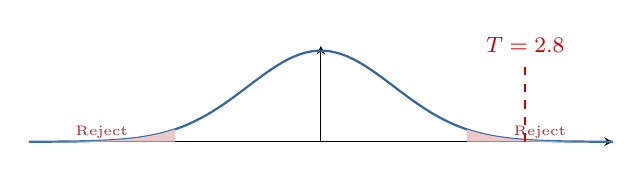
\begin{tikzpicture}
  \begin{axis}[
    width=9cm, height=2.8cm,
    domain=-4:4, samples=100,
    axis lines=middle, ticks=none,
    ymin=0, ymax=0.42,
    every axis plot/.style={thick, no markers},
    clip=false
  ]
    \addplot[popblue, thick] {exp(-0.5*x^2) / sqrt(2*pi)};
    \addplot[fill=warnred!25, draw=none, domain=-4:-2] {exp(-0.5*x^2) / sqrt(2*pi)} \closedcycle;
    \addplot[fill=warnred!25, draw=none, domain=2:4] {exp(-0.5*x^2) / sqrt(2*pi)} \closedcycle;
    \draw[thick, dashed, sampred] (axis cs:2.8, 0) -- (axis cs:2.8, 0.35);
    \node[font=\footnotesize\bfseries, sampred, above] at (axis cs:2.8, 0.35) {$T = 2.8$};
    \node[font=\tiny, warnred] at (axis cs:-3, 0.04) {Reject};
    \node[font=\tiny, warnred] at (axis cs:3, 0.04) {Reject};
  \end{axis}
\end{tikzpicture}
\end{center}

\vspace{0.1cm}
\small
\textbf{Interpretation:} ``Is this predictor useful, \textit{controlling for} all others in the model?''\\
$H_0\!: \beta_j = 0$ means $X_j$ has no linear effect on $Y$ after accounting for other predictors.
\end{frame}

\begin{frame}
\frametitle{Example: Predicting House Prices}

\small
$n = 100$ houses. Model: Price $= \beta_0 + \beta_1 \cdot \text{Size} + \beta_2 \cdot \text{Bedrooms} + \beta_3 \cdot \text{Age} + \varepsilon$.

\vspace{0.15cm}
\begin{center}
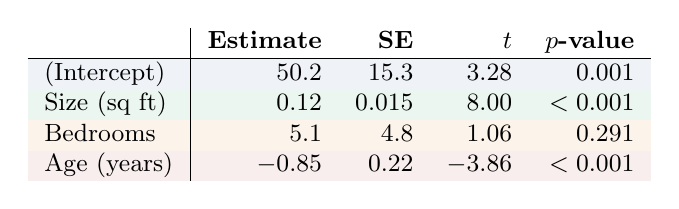
\begin{tikzpicture}
  \node[inner sep=0pt] {
    \small
    \begin{tabular}{l|rrrr}
      & \textbf{Estimate} & \textbf{SE} & \textbf{$t$} & \textbf{$p$-value} \\
      \hline
      \rowcolor{popblue!8}
      (Intercept) & 50.2 & 15.3 & 3.28 & 0.001 \\
      \rowcolor{paramgreen!8}
      Size (sq ft) & 0.12 & 0.015 & 8.00 & $< 0.001$ \\
      \rowcolor{orange1!8}
      Bedrooms & 5.1 & 4.8 & 1.06 & 0.291 \\
      \rowcolor{warnred!8}
      Age (years) & $-0.85$ & 0.22 & $-3.86$ & $< 0.001$ \\
    \end{tabular}
  };
\end{tikzpicture}
\end{center}

\vspace{0.15cm}
\begin{center}
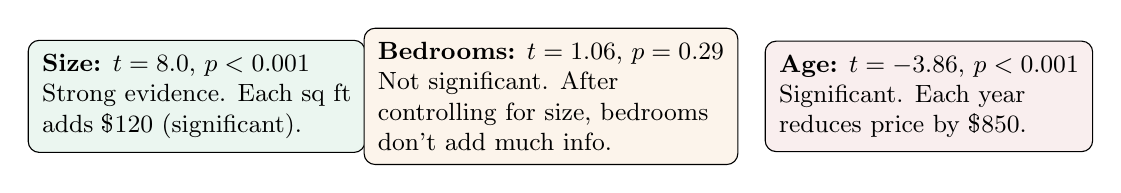
\begin{tikzpicture}[
  ibox/.style={draw, rounded corners=4pt, inner sep=5pt, font=\small, align=left}
]
  \node[ibox, fill=paramgreen!8] at (-4.5, 0) {
    \textbf{Size:} $t = 8.0$, $p < 0.001$\\
    Strong evidence. Each sq ft\\
    adds \$120 (significant).
  };
  \node[ibox, fill=orange1!8] at (0, 0) {
    \textbf{Bedrooms:} $t = 1.06$, $p = 0.29$\\
    Not significant. After\\
    controlling for size, bedrooms\\
    don't add much info.
  };
  \node[ibox, fill=warnred!8] at (4.8, 0) {
    \textbf{Age:} $t = -3.86$, $p < 0.001$\\
    Significant. Each year\\
    reduces price by \$850.
  };
\end{tikzpicture}
\end{center}
\end{frame}

\begin{frame}
\frametitle{Confidence Intervals for Coefficients}

\begin{center}
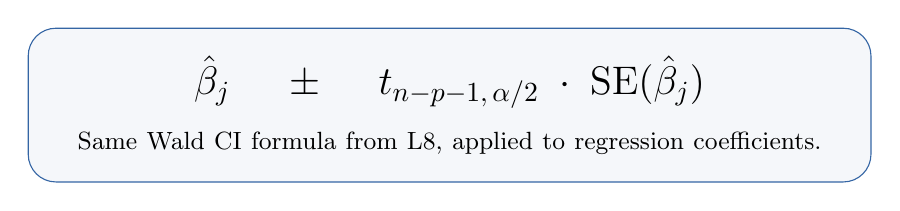
\begin{tikzpicture}
  \node[draw=popblue, fill=popblue!5, rounded corners=10pt, text width=10cm, align=center, inner sep=10pt] {
    {\Large $\hat{\beta}_j \;\pm\; t_{n-p-1,\,\alpha/2} \cdot \text{SE}(\hat{\beta}_j)$}\\[8pt]
    \small Same Wald CI formula from L8, applied to regression coefficients.
  };
\end{tikzpicture}
\end{center}

\vspace{0.2cm}
\textbf{House price example} (95\% CI, $t_{96, 0.025} \approx 1.985$):

\vspace{0.1cm}
\begin{center}
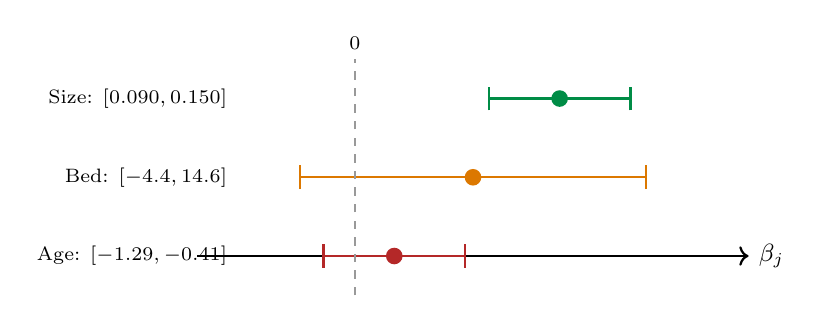
\begin{tikzpicture}
  % CI visualization
  \draw[thick, ->] (-1, 0) -- (6, 0) node[right, font=\small] {$\beta_j$};

  % Size
  \fill[paramgreen] (3.6, 2) circle (3pt);
  \draw[thick, paramgreen] (2.7, 2) -- (4.5, 2);
  \draw[thick, paramgreen] (2.7, 1.85) -- (2.7, 2.15);
  \draw[thick, paramgreen] (4.5, 1.85) -- (4.5, 2.15);
  \node[font=\scriptsize, left] at (-0.5, 2) {Size: $[0.090, 0.150]$};

  % Bedrooms
  \fill[orange1] (2.5, 1) circle (3pt);
  \draw[thick, orange1] (0.3, 1) -- (4.7, 1);
  \draw[thick, orange1] (0.3, 0.85) -- (0.3, 1.15);
  \draw[thick, orange1] (4.7, 0.85) -- (4.7, 1.15);
  \node[font=\scriptsize, left] at (-0.5, 1) {Bed: $[-4.4, 14.6]$};

  % Age
  \fill[warnred] (1.5, 0) circle (3pt);
  \draw[thick, warnred] (0.6, 0) -- (2.4, 0);
  \draw[thick, warnred] (0.6, -0.15) -- (0.6, 0.15);
  \draw[thick, warnred] (2.4, -0.15) -- (2.4, 0.15);
  \node[font=\scriptsize, left] at (-0.5, 0) {Age: $[-1.29, -0.41]$};

  % Zero line
  \draw[thick, dashed, black!40] (1, -0.5) -- (1, 2.5);
  \node[font=\scriptsize, above] at (1, 2.5) {$0$};
\end{tikzpicture}
\end{center}

\vspace{0.1cm}
\small Bedrooms CI contains 0 $\Rightarrow$ not significant. Size and Age CIs exclude 0 $\Rightarrow$ significant.\\
\textbf{CI and $p$-value always agree:} CI contains 0 $\Leftrightarrow$ $p > \alpha$.
\end{frame}

% ============================================================
% PART III: THE OVERALL F-TEST & R²
% ============================================================
\section{Overall Model Fit}

\begin{frame}
\begin{center}
  \vspace{1.5cm}
  {\Huge\bfseries\textcolor{popblue}{Part III: Overall Model Fit}}

  \vspace{0.8cm}
  {\large Is the model as a whole useful? How much does it explain?}
\end{center}
\end{frame}

\begin{frame}
\frametitle{The Overall $F$-Test}
\framesubtitle{Tests whether \textit{any} predictor is useful}

\begin{center}
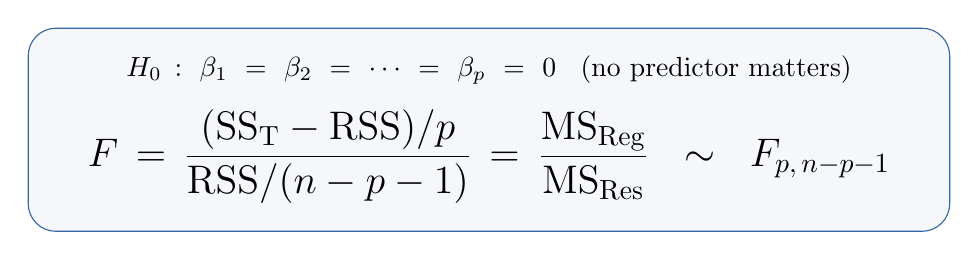
\begin{tikzpicture}
  \node[draw=popblue, fill=popblue!5, rounded corners=10pt, text width=11cm, align=center, inner sep=10pt] {
    $H_0\!: \beta_1 = \beta_2 = \cdots = \beta_p = 0$ \;\;(no predictor matters)\\[8pt]
    {\Large $F = \dfrac{(\text{SS}_\text{T} - \text{RSS})/p}{\text{RSS}/(n - p - 1)} = \dfrac{\text{MS}_\text{Reg}}{\text{MS}_\text{Res}} \;\sim\; F_{p,\,n-p-1}$}
  };
\end{tikzpicture}
\end{center}

\vspace{0.2cm}
\begin{center}
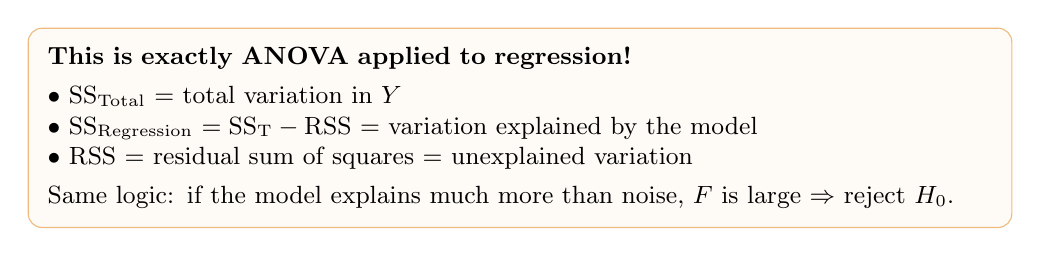
\begin{tikzpicture}
  \node[draw=orange1!50, fill=orange1!3, rounded corners=5pt, text width=12cm, align=left, inner sep=7pt, font=\small] {
    \textbf{This is exactly ANOVA applied to regression!}\\[3pt]
    $\bullet$ SS\textsubscript{Total} = total variation in $Y$\\
    $\bullet$ SS\textsubscript{Regression} $= \text{SS}_\text{T} - \text{RSS}$ = variation explained by the model\\
    $\bullet$ RSS = residual sum of squares = unexplained variation\\[3pt]
    Same logic: if the model explains much more than noise, $F$ is large $\Rightarrow$ reject $H_0$.
  };
\end{tikzpicture}
\end{center}

\vspace{0.1cm}
\begin{center}
\small \textbf{House prices:} $F = 85.3$ on 3 and 96 df, $p < 0.001$. The model is highly significant.
\end{center}
\end{frame}

\begin{frame}
\frametitle{$R^2$ and Adjusted $R^2$}

\begin{center}
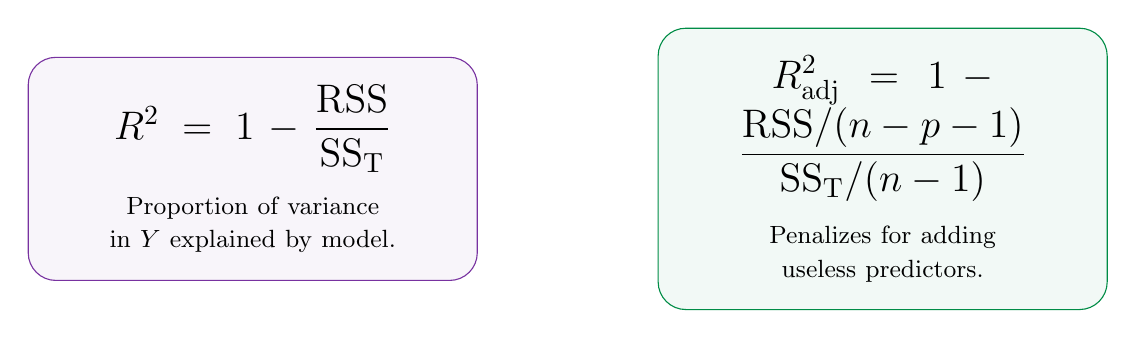
\begin{tikzpicture}
  \node[draw=violet1, fill=violet1!5, rounded corners=10pt, text width=5cm, align=center, inner sep=10pt] at (-4, 0) {
    {\Large $R^2 = 1 - \dfrac{\text{RSS}}{\text{SS}_\text{T}}$}\\[8pt]
    \small Proportion of variance\\
    in $Y$ explained by model.
  };
  \node[draw=paramgreen, fill=paramgreen!5, rounded corners=10pt, text width=5cm, align=center, inner sep=10pt] at (4, 0) {
    {\Large $R^2_{\text{adj}} = 1 - \dfrac{\text{RSS}/(n-p-1)}{\text{SS}_\text{T}/(n-1)}$}\\[8pt]
    \small Penalizes for adding\\
    useless predictors.
  };
\end{tikzpicture}
\end{center}

\vspace{0.3cm}
\begin{center}
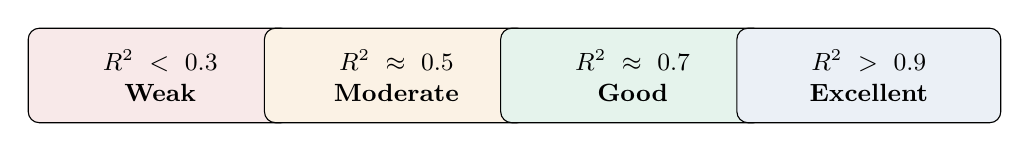
\begin{tikzpicture}[
  rbox/.style={draw, rounded corners=4pt, text width=3cm, align=center, inner sep=5pt, font=\small, minimum height=1.2cm}
]
  \node[rbox, fill=warnred!10] at (-4.5, 0) {$R^2 < 0.3$\\\textbf{Weak}};
  \node[rbox, fill=orange1!10] at (-1.5, 0) {$R^2 \approx 0.5$\\\textbf{Moderate}};
  \node[rbox, fill=paramgreen!10] at (1.5, 0) {$R^2 \approx 0.7$\\\textbf{Good}};
  \node[rbox, fill=popblue!10] at (4.5, 0) {$R^2 > 0.9$\\\textbf{Excellent}};
\end{tikzpicture}
\end{center}

\vspace{0.15cm}
\begin{center}
\fcolorbox{warnred}{warnred!5}{\parbox{10cm}{\centering\footnotesize
  \textbf{Trap:} $R^2$ \textit{always} increases when you add predictors, even useless ones.\\
  Use $R^2_\text{adj}$ to compare models with different numbers of predictors.\\
  ``I got $R^2 = 0.95$'' means nothing if you have $n = 20$ and $p = 18$.
}}
\end{center}
\end{frame}

% ============================================================
% PART IV: GAUSS-MARKOV
% ============================================================
\section{Gauss--Markov Theorem}

\begin{frame}
\begin{center}
  \vspace{1.5cm}
  {\Huge\bfseries\textcolor{popblue}{Part IV: Why OLS?}}

  \vspace{0.8cm}
  {\large The Gauss--Markov theorem: OLS is the best you can do (with conditions)}
\end{center}
\end{frame}

\begin{frame}
\frametitle{The Gauss--Markov Theorem}

\begin{center}
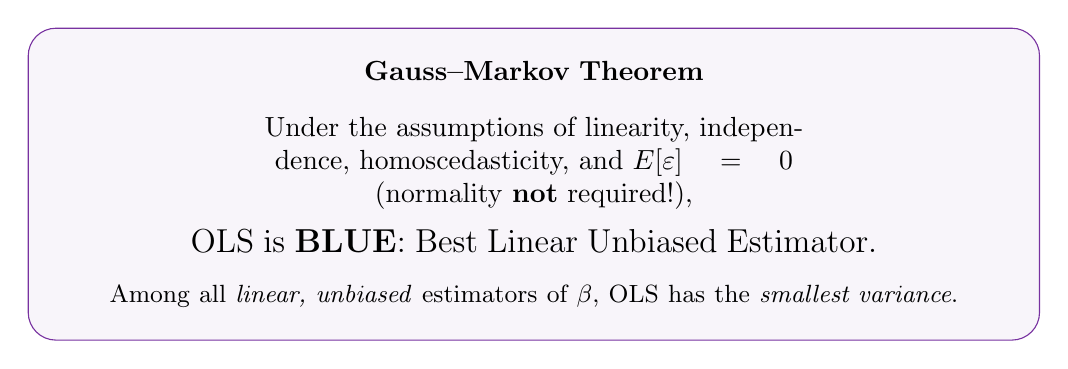
\begin{tikzpicture}
  \node[draw=violet1, fill=violet1!5, rounded corners=10pt, text width=12cm, align=center, inner sep=12pt] {
    \textbf{Gauss--Markov Theorem}\\[8pt]
    Under the assumptions of linearity, independence, homoscedasticity, and $E[\varepsilon] = 0$\\
    (normality \textbf{not} required!),\\[6pt]
    {\large OLS is \textbf{BLUE}: Best Linear Unbiased Estimator.}\\[6pt]
    \small Among all \textit{linear, unbiased} estimators of $\beta$, OLS has the \textit{smallest variance}.
  };
\end{tikzpicture}
\end{center}

\vspace{0.3cm}
\begin{center}
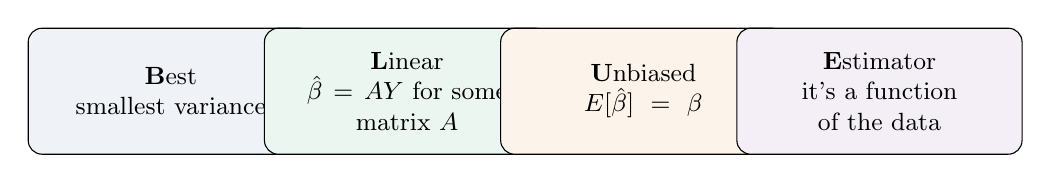
\begin{tikzpicture}[
  cbox/.style={draw, rounded corners=5pt, text width=3.2cm, align=center, inner sep=6pt, font=\small, minimum height=1.6cm}
]
  \node[cbox, fill=popblue!8] at (-4.5, 0) {\textbf{B}est\\smallest variance};
  \node[cbox, fill=paramgreen!8] at (-1.5, 0) {\textbf{L}inear\\$\hat\beta = AY$ for some\\matrix $A$};
  \node[cbox, fill=orange1!8] at (1.5, 0) {\textbf{U}nbiased\\$E[\hat\beta] = \beta$};
  \node[cbox, fill=violet1!8] at (4.5, 0) {\textbf{E}stimator\\it's a function\\of the data};
\end{tikzpicture}
\end{center}

\vspace{0.1cm}
\begin{center}
\small\textit{Connects to L3:} among unbiased estimators, lowest variance = best. Same principle as Cram\'er--Rao.
\end{center}
\end{frame}

\begin{frame}
\frametitle{When Gauss--Markov Doesn't Help}

\begin{center}
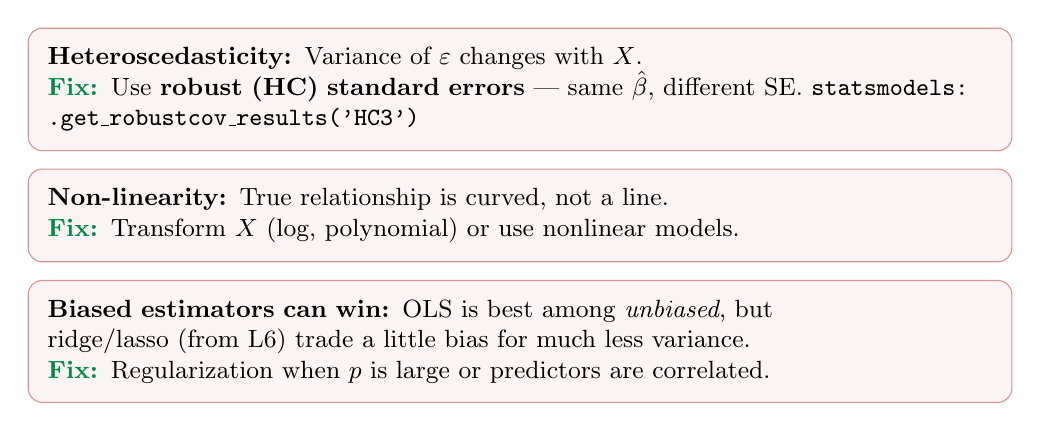
\begin{tikzpicture}[
  pbox/.style={draw=warnred!50, fill=warnred!5, rounded corners=5pt, text width=12cm, align=left, inner sep=7pt, font=\small}
]
  \node[pbox] at (0, 2.4) {
    \textbf{Heteroscedasticity:} Variance of $\varepsilon$ changes with $X$.\\
    \textcolor{paramgreen}{\textbf{Fix:}} Use \textbf{robust (HC) standard errors} --- same $\hat\beta$, different SE.
    \texttt{statsmodels: .get\_robustcov\_results('HC3')}
  };
  \node[pbox] at (0, 0.8) {
    \textbf{Non-linearity:} True relationship is curved, not a line.\\
    \textcolor{paramgreen}{\textbf{Fix:}} Transform $X$ (log, polynomial) or use nonlinear models.
  };
  \node[pbox] at (0, -0.8) {
    \textbf{Biased estimators can win:} OLS is best among \textit{unbiased}, but\\
    ridge/lasso (from L6) trade a little bias for much less variance.\\
    \textcolor{paramgreen}{\textbf{Fix:}} Regularization when $p$ is large or predictors are correlated.
  };
\end{tikzpicture}
\end{center}

\vspace{0.15cm}
\begin{center}
\fcolorbox{orange1}{orange1!5}{\parbox{10cm}{\centering\footnotesize
  Gauss--Markov says OLS is the best \textit{unbiased linear} estimator.\\
  It does \textbf{not} say OLS is the best estimator, period. (Recall L3: bias-variance tradeoff.)
}}
\end{center}
\end{frame}

% ============================================================
% PART V: DIAGNOSTICS
% ============================================================
\section{Regression Diagnostics}

\begin{frame}
\begin{center}
  \vspace{1.5cm}
  {\Huge\bfseries\textcolor{popblue}{Part V: Diagnostics}}

  \vspace{0.8cm}
  {\large How to check if your model's assumptions hold}
\end{center}
\end{frame}

\begin{frame}
\frametitle{The Four Diagnostic Plots}

\begin{center}
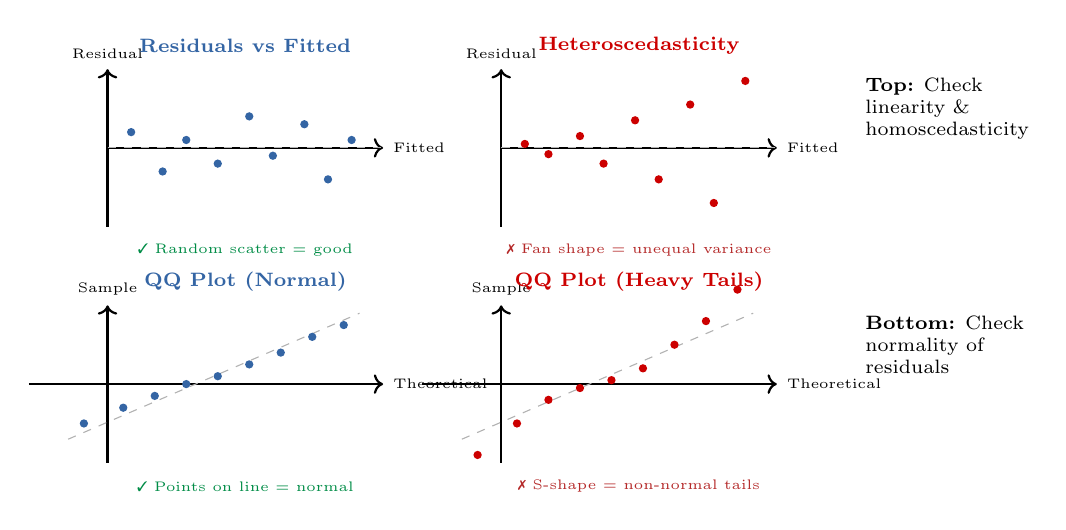
\begin{tikzpicture}
  % Plot 1: Residuals vs Fitted (good)
  \begin{scope}[shift={(0, 3)}]
    \draw[thick, ->] (0, 0) -- (3.5, 0) node[right, font=\tiny] {Fitted};
    \draw[thick, ->] (0, -1) -- (0, 1) node[above, font=\tiny] {Residual};
    \draw[dashed, black!30] (0, 0) -- (3.5, 0);
    \foreach \x/\y in {0.3/0.2, 0.7/-0.3, 1.0/0.1, 1.4/-0.2, 1.8/0.4, 2.1/-0.1, 2.5/0.3, 2.8/-0.4, 3.1/0.1} {
      \fill[popblue] (\x, \y) circle (1.5pt);
    }
    \node[font=\scriptsize\bfseries, popblue] at (1.75, 1.3) {Residuals vs Fitted};
    \node[font=\tiny, paramgreen] at (1.75, -1.3) {\ding{51} Random scatter = good};
  \end{scope}

  % Plot 2: Residuals vs Fitted (bad - funnel)
  \begin{scope}[shift={(5, 3)}]
    \draw[thick, ->] (0, 0) -- (3.5, 0) node[right, font=\tiny] {Fitted};
    \draw[thick, ->] (0, -1) -- (0, 1) node[above, font=\tiny] {Residual};
    \draw[dashed, black!30] (0, 0) -- (3.5, 0);
    \foreach \x/\y in {0.3/0.05, 0.6/-0.08, 1.0/0.15, 1.3/-0.2, 1.7/0.35, 2.0/-0.4, 2.4/0.55, 2.7/-0.7, 3.1/0.85} {
      \fill[sampred] (\x, \y) circle (1.5pt);
    }
    \node[font=\scriptsize\bfseries, sampred] at (1.75, 1.3) {Heteroscedasticity};
    \node[font=\tiny, warnred] at (1.75, -1.3) {\ding{55} Fan shape = unequal variance};
  \end{scope}

  % Plot 3: QQ plot (good)
  \begin{scope}[shift={(0, 0)}]
    \draw[thick, ->] (0, -1) -- (0, 1) node[above, font=\tiny] {Sample};
    \draw[thick, ->] (-1, 0) -- (3.5, 0) node[right, font=\tiny] {Theoretical};
    \draw[dashed, black!30] (-0.5, -0.7) -- (3.2, 0.9);
    \foreach \x/\y in {-0.3/-0.5, 0.2/-0.3, 0.6/-0.15, 1.0/0.0, 1.4/0.1, 1.8/0.25, 2.2/0.4, 2.6/0.6, 3.0/0.75} {
      \fill[popblue] (\x, \y) circle (1.5pt);
    }
    \node[font=\scriptsize\bfseries, popblue] at (1.75, 1.3) {QQ Plot (Normal)};
    \node[font=\tiny, paramgreen] at (1.75, -1.3) {\ding{51} Points on line = normal};
  \end{scope}

  % Plot 4: QQ plot (bad - heavy tails)
  \begin{scope}[shift={(5, 0)}]
    \draw[thick, ->] (0, -1) -- (0, 1) node[above, font=\tiny] {Sample};
    \draw[thick, ->] (-1, 0) -- (3.5, 0) node[right, font=\tiny] {Theoretical};
    \draw[dashed, black!30] (-0.5, -0.7) -- (3.2, 0.9);
    \foreach \x/\y in {-0.3/-0.9, 0.2/-0.5, 0.6/-0.2, 1.0/-0.05, 1.4/0.05, 1.8/0.2, 2.2/0.5, 2.6/0.8, 3.0/1.2} {
      \fill[sampred] (\x, \y) circle (1.5pt);
    }
    \node[font=\scriptsize\bfseries, sampred] at (1.75, 1.3) {QQ Plot (Heavy Tails)};
    \node[font=\tiny, warnred] at (1.75, -1.3) {\ding{55} S-shape = non-normal tails};
  \end{scope}

  % Plot labels
  \node[font=\scriptsize, right, align=left] at (9.5, 3.5) {\textbf{Top:} Check\\linearity \&\\homoscedasticity};
  \node[font=\scriptsize, right, align=left] at (9.5, 0.5) {\textbf{Bottom:} Check\\normality of\\residuals};
\end{tikzpicture}
\end{center}
\end{frame}

\begin{frame}
\frametitle{Leverage and Influential Points}

\begin{center}
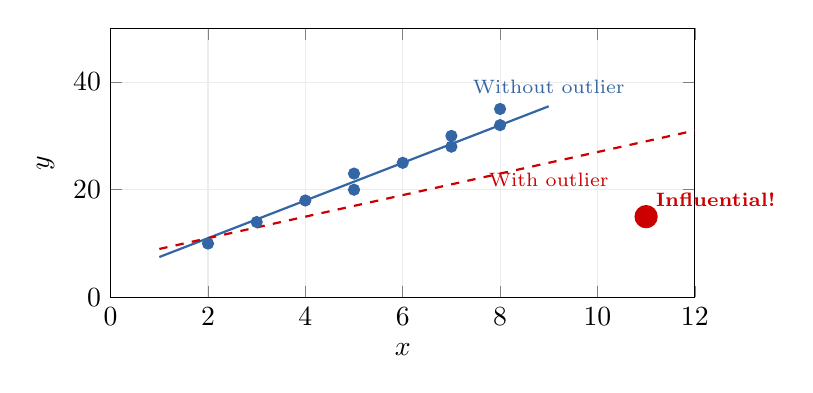
\begin{tikzpicture}
  \begin{axis}[
    width=9cm, height=5cm,
    xlabel={$x$}, ylabel={$y$},
    xmin=0, xmax=12, ymin=0, ymax=50,
    grid=major, grid style={gray!15},
    clip=false
  ]
    % Normal points
    \addplot[only marks, mark=*, mark size=2pt, popblue] coordinates {
      (2,10) (3,14) (4,18) (5,20) (5,23) (6,25) (7,28) (7,30) (8,32) (8,35)
    };
    % Regression without outlier
    \addplot[popblue, thick, domain=1:9] {4 + 3.5*x};
    \node[font=\scriptsize, popblue, above] at (axis cs:9, 36) {Without outlier};

    % Influential point
    \addplot[only marks, mark=*, mark size=4pt, sampred] coordinates {(11, 15)};
    \node[font=\scriptsize\bfseries, sampred, above right] at (axis cs:11, 15) {Influential!};

    % Regression with outlier
    \addplot[sampred, thick, dashed, domain=1:12] {7 + 2*x};
    \node[font=\scriptsize, sampred, below] at (axis cs:9, 25) {With outlier};
  \end{axis}
\end{tikzpicture}
\end{center}

\vspace{0.05cm}
\begin{center}
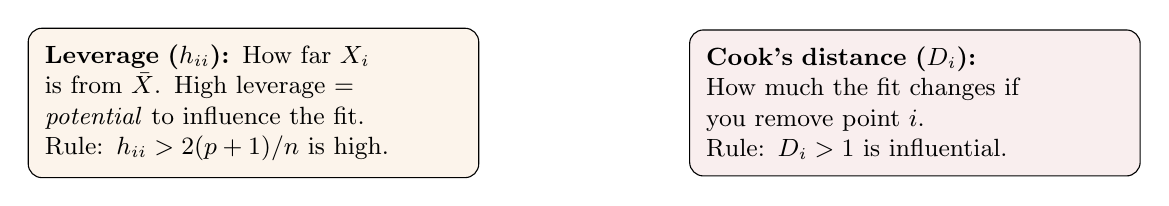
\begin{tikzpicture}[
  cbox/.style={draw, rounded corners=5pt, text width=5.3cm, align=left, inner sep=6pt, font=\small}
]
  \node[cbox, fill=orange1!8] at (-4.2, 0) {
    \textbf{Leverage ($h_{ii}$):} How far $X_i$\\
    is from $\bar{X}$. High leverage =\\
    \textit{potential} to influence the fit.\\
    Rule: $h_{ii} > 2(p+1)/n$ is high.
  };
  \node[cbox, fill=warnred!8] at (4.2, 0) {
    \textbf{Cook's distance ($D_i$):}\\
    How much the fit changes if\\
    you remove point $i$.\\
    Rule: $D_i > 1$ is influential.
  };
\end{tikzpicture}
\end{center}
\end{frame}

% ============================================================
% PART VI: LOGISTIC REGRESSION INFERENCE
% ============================================================
\section{Logistic Regression Inference}

\begin{frame}
\begin{center}
  \vspace{1.5cm}
  {\Huge\bfseries\textcolor{popblue}{Part VI: Logistic Regression}}

  \vspace{0.8cm}
  {\large When $Y$ is binary: from MLE to inference}
\end{center}
\end{frame}

\begin{frame}
\frametitle{Logistic Regression as MLE}
\framesubtitle{Connects to L5 (MLE) and L6 (cross-entropy)}

\vspace{-0.1cm}
\begin{center}
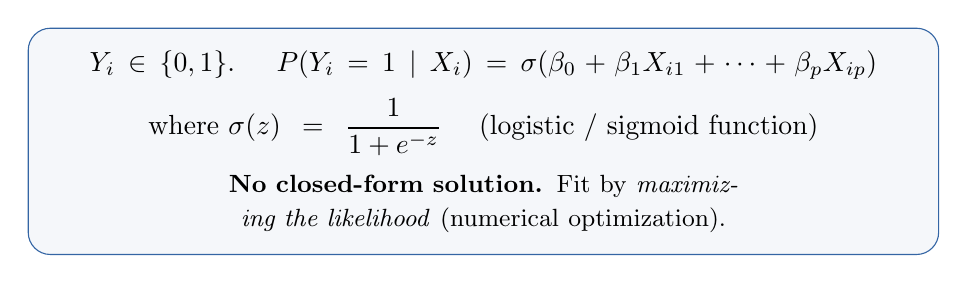
\begin{tikzpicture}
  \node[draw=popblue, fill=popblue!5, rounded corners=8pt, text width=11cm, align=center, inner sep=8pt] {
    $Y_i \in \{0, 1\}$. \quad
    $P(Y_i = 1 \mid X_i) = \sigma(\beta_0 + \beta_1 X_{i1} + \cdots + \beta_p X_{ip})$\\[6pt]
    where $\sigma(z) = \dfrac{1}{1 + e^{-z}}$ \quad (logistic / sigmoid function)\\[6pt]
    \small \textbf{No closed-form solution.} Fit by \textit{maximizing the likelihood} (numerical optimization).
  };
\end{tikzpicture}
\end{center}

\vspace{0.1cm}
\begin{center}
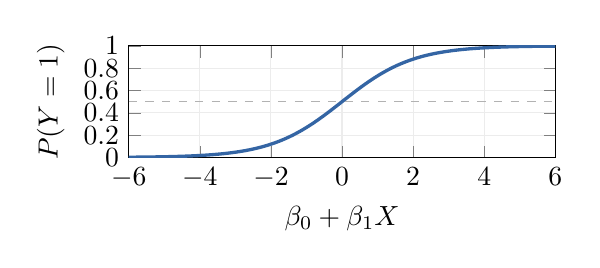
\begin{tikzpicture}
  \begin{axis}[
    width=7cm, height=3cm,
    domain=-6:6, samples=100,
    xlabel={$\beta_0 + \beta_1 X$},
    ylabel={$P(Y=1)$},
    xmin=-6, xmax=6, ymin=0, ymax=1,
    grid=major, grid style={gray!15},
    every axis plot/.style={thick, no markers}
  ]
    \addplot[popblue, very thick] {1/(1+exp(-x))};
    \draw[dashed, black!30] (axis cs:-6, 0.5) -- (axis cs:6, 0.5);
  \end{axis}
\end{tikzpicture}
\end{center}

\vspace{0.05cm}
\begin{center}
\small The negative log-likelihood is the \textbf{cross-entropy loss} from L5. MLE = minimize cross-entropy.
\end{center}
\end{frame}

\begin{frame}
\frametitle{Inference for Logistic Regression}

\begin{center}
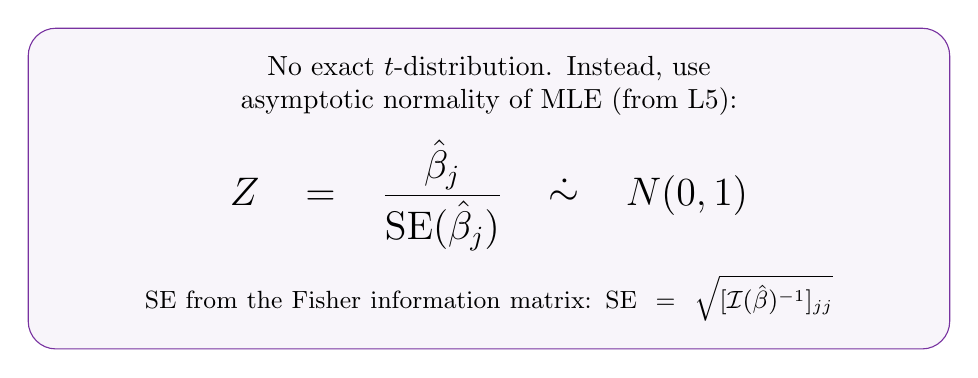
\begin{tikzpicture}
  \node[draw=violet1, fill=violet1!5, rounded corners=10pt, text width=11cm, align=center, inner sep=10pt] {
    No exact $t$-distribution. Instead, use asymptotic normality of MLE (from L5):\\[8pt]
    {\Large $Z = \dfrac{\hat{\beta}_j}{\text{SE}(\hat{\beta}_j)} \;\dot{\sim}\; N(0, 1)$}\\[8pt]
    \small SE from the Fisher information matrix: $\text{SE} = \sqrt{[\mathcal{I}(\hat\beta)^{-1}]_{jj}}$
  };
\end{tikzpicture}
\end{center}

\vspace{0.2cm}
\textbf{Example:} Predicting college admission ($Y$) from GPA ($X_1$) and test score ($X_2$).

\vspace{0.1cm}
\begin{center}
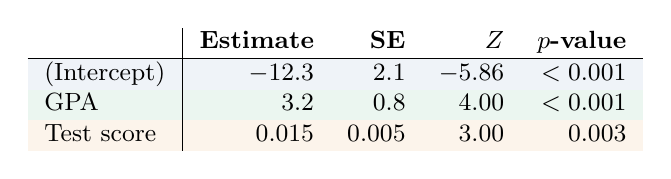
\begin{tikzpicture}
  \node[inner sep=0pt] {
    \small
    \begin{tabular}{l|rrrr}
      & \textbf{Estimate} & \textbf{SE} & \textbf{$Z$} & \textbf{$p$-value} \\
      \hline
      \rowcolor{popblue!8}
      (Intercept) & $-12.3$ & 2.1 & $-5.86$ & $< 0.001$ \\
      \rowcolor{paramgreen!8}
      GPA & 3.2 & 0.8 & 4.00 & $< 0.001$ \\
      \rowcolor{orange1!8}
      Test score & 0.015 & 0.005 & 3.00 & 0.003 \\
    \end{tabular}
  };
\end{tikzpicture}
\end{center}

\vspace{0.1cm}
\small Both GPA and test score are significant predictors of admission.
\end{frame}

\begin{frame}
\frametitle{Interpreting Logistic Coefficients: Odds Ratios}

\begin{center}
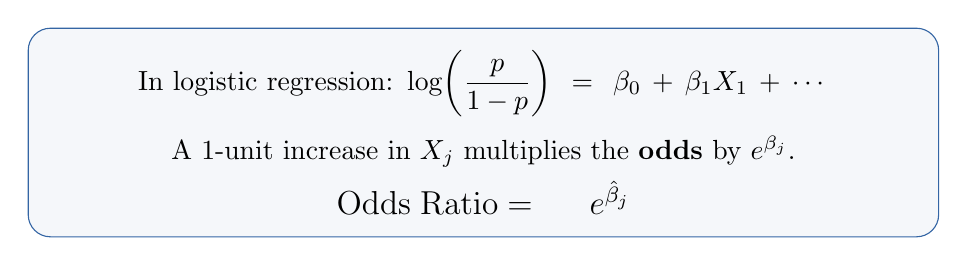
\begin{tikzpicture}
  \node[draw=popblue, fill=popblue!5, rounded corners=8pt, text width=11cm, align=center, inner sep=8pt] {
    In logistic regression: $\log\!\left(\dfrac{p}{1-p}\right) = \beta_0 + \beta_1 X_1 + \cdots$\\[6pt]
    A 1-unit increase in $X_j$ multiplies the \textbf{odds} by $e^{\beta_j}$.\\[4pt]
    {\large Odds Ratio $= e^{\hat{\beta}_j}$}
  };
\end{tikzpicture}
\end{center}

\vspace{0.1cm}
\textbf{Admission example:}

\vspace{0.05cm}
\begin{center}
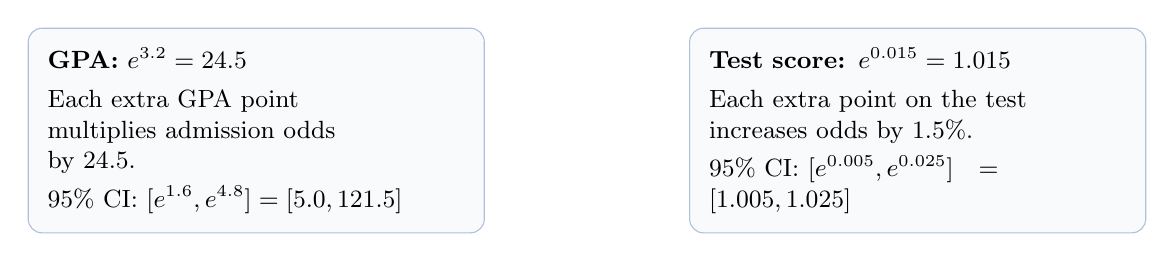
\begin{tikzpicture}[
  obox/.style={draw=popblue!40, fill=popblue!3, rounded corners=5pt, text width=5.3cm, align=left, inner sep=7pt, font=\small}
]
  \node[obox] at (-4.2, 0) {
    \textbf{GPA:} $e^{3.2} = 24.5$\\[3pt]
    Each extra GPA point\\
    multiplies admission odds\\
    by 24.5.\\[3pt]
    95\% CI: $[e^{1.6}, e^{4.8}] = [5.0, 121.5]$
  };
  \node[obox] at (4.2, 0) {
    \textbf{Test score:} $e^{0.015} = 1.015$\\[3pt]
    Each extra point on the test\\
    increases odds by 1.5\%.\\[3pt]
    95\% CI: $[e^{0.005}, e^{0.025}] = [1.005, 1.025]$
  };
\end{tikzpicture}
\end{center}

\vspace{0.1cm}
\begin{center}
\small OR $> 1$: increases odds. OR $< 1$: decreases odds. OR $= 1$: no effect.
\end{center}
\end{frame}

\begin{frame}
\frametitle{OLS vs Logistic: Side by Side}

\begin{center}
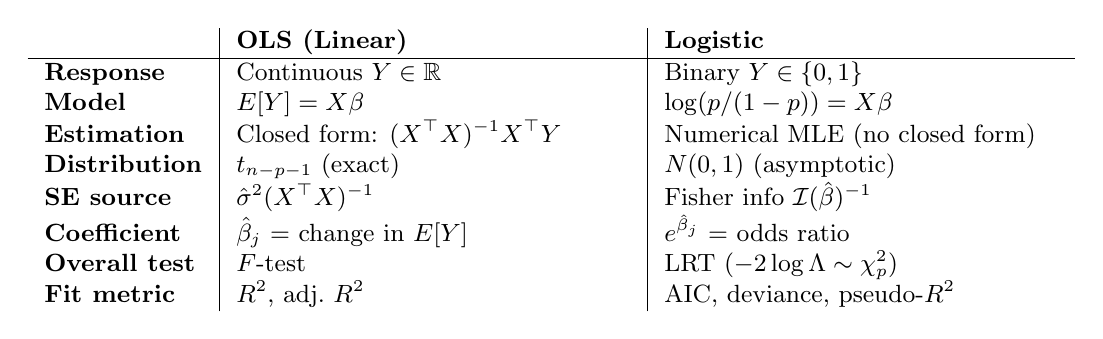
\begin{tikzpicture}
  \node[inner sep=0pt] {
    \small
    \begin{tabular}{l|p{5cm}|p{5cm}}
      & \textbf{OLS (Linear)} & \textbf{Logistic} \\
      \hline
      \textbf{Response} & Continuous $Y \in \mathbb{R}$ & Binary $Y \in \{0,1\}$ \\
      \textbf{Model} & $E[Y] = X\beta$ & $\log(p/(1-p)) = X\beta$ \\
      \textbf{Estimation} & Closed form: $(X^\top X)^{-1}X^\top Y$ & Numerical MLE (no closed form) \\
      \textbf{Distribution} & $t_{n-p-1}$ (exact) & $N(0,1)$ (asymptotic) \\
      \textbf{SE source} & $\hat\sigma^2 (X^\top X)^{-1}$ & Fisher info $\mathcal{I}(\hat\beta)^{-1}$ \\
      \textbf{Coefficient} & $\hat\beta_j$ = change in $E[Y]$ & $e^{\hat\beta_j}$ = odds ratio \\
      \textbf{Overall test} & $F$-test & LRT ($-2\log\Lambda \sim \chi^2_p$) \\
      \textbf{Fit metric} & $R^2$, adj.\ $R^2$ & AIC, deviance, pseudo-$R^2$ \\
    \end{tabular}
  };
\end{tikzpicture}
\end{center}

\vspace{0.2cm}
\begin{center}
\fcolorbox{popblue}{popblue!5}{\parbox{10cm}{\centering\small
  \textbf{Same workflow:} Fit model $\to$ check significance of each $\hat\beta_j$ $\to$ check overall fit $\to$ diagnostics.\\
  The tools change (exact $t$ vs asymptotic $Z$, $R^2$ vs deviance), but the logic is identical.
}}
\end{center}
\end{frame}

% ============================================================
\section{Summary}

\begin{frame}
\frametitle{Summary: Regression Inference}
\begin{center}
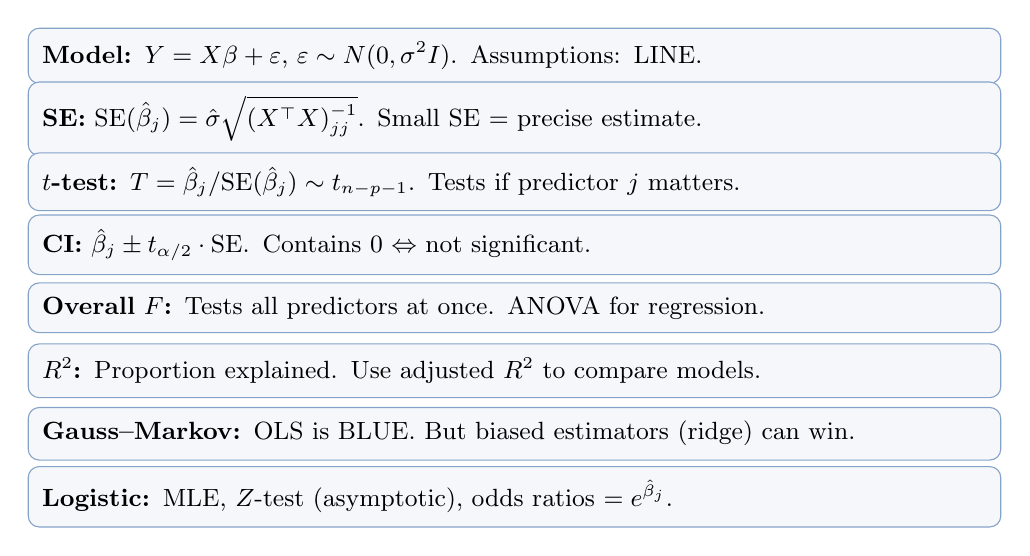
\begin{tikzpicture}[
  sbox/.style={draw=popblue!60, fill=popblue!5, rounded corners=4pt, text width=12cm, minimum height=0.5cm, align=left, inner sep=5pt, font=\small}
]
  \node[sbox] at (0, 3.2) {\textbf{Model:} $Y = X\beta + \varepsilon$, $\varepsilon \sim N(0, \sigma^2 I)$. Assumptions: LINE.};
  \node[sbox] at (0, 2.4) {\textbf{SE:} $\text{SE}(\hat\beta_j) = \hat\sigma\sqrt{(X^\top X)^{-1}_{jj}}$. Small SE = precise estimate.};
  \node[sbox] at (0, 1.6) {\textbf{$t$-test:} $T = \hat\beta_j / \text{SE}(\hat\beta_j) \sim t_{n-p-1}$. Tests if predictor $j$ matters.};
  \node[sbox] at (0, 0.8) {\textbf{CI:} $\hat\beta_j \pm t_{\alpha/2} \cdot \text{SE}$. Contains 0 $\Leftrightarrow$ not significant.};
  \node[sbox] at (0, 0.0) {\textbf{Overall $F$:} Tests all predictors at once. ANOVA for regression.};
  \node[sbox] at (0, -0.8) {\textbf{$R^2$:} Proportion explained. Use adjusted $R^2$ to compare models.};
  \node[sbox] at (0, -1.6) {\textbf{Gauss--Markov:} OLS is BLUE. But biased estimators (ridge) can win.};
  \node[sbox] at (0, -2.4) {\textbf{Logistic:} MLE, $Z$-test (asymptotic), odds ratios $= e^{\hat\beta_j}$.};
\end{tikzpicture}
\end{center}
\end{frame}

% ============================================================
\section{Practical}

\begin{frame}
\frametitle{Practical: Regression Inference in Python}
\begin{center}
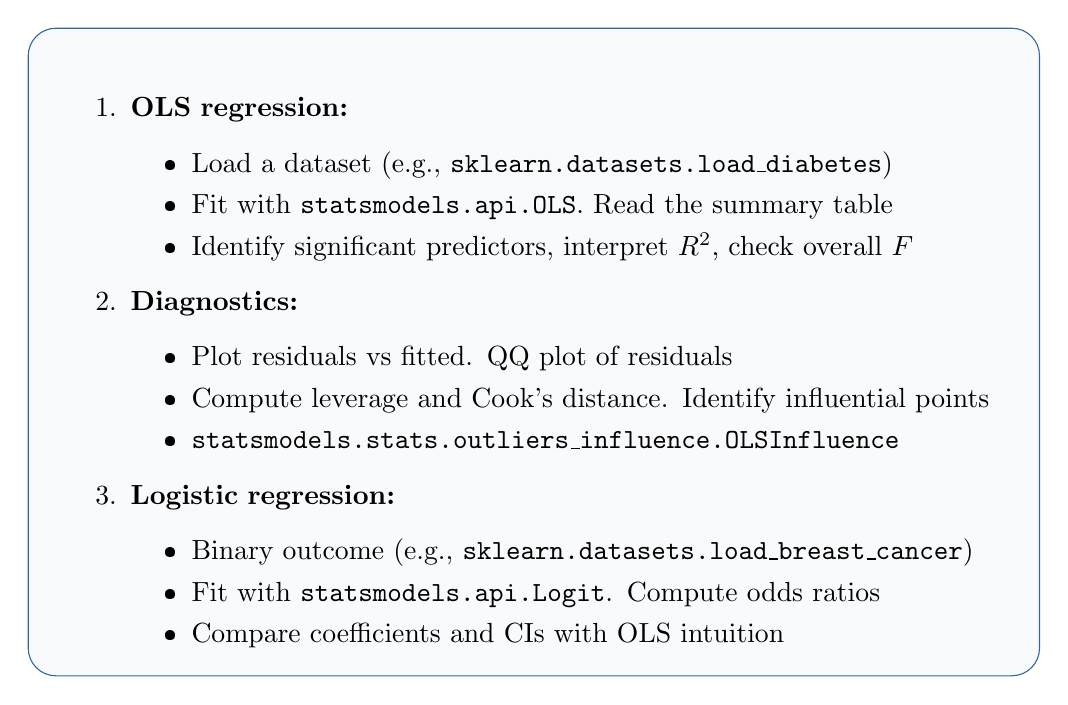
\begin{tikzpicture}
  \node[draw=popblue, fill=popblue!3, rounded corners=10pt, text width=12cm, align=left, inner sep=12pt] {
    \begin{enumerate}\setlength{\itemsep}{4pt}
      \item \textbf{OLS regression:}
        \begin{itemize}\setlength{\itemsep}{1pt}
          \item Load a dataset (e.g., \texttt{sklearn.datasets.load\_diabetes})
          \item Fit with \texttt{statsmodels.api.OLS}. Read the summary table
          \item Identify significant predictors, interpret $R^2$, check overall $F$
        \end{itemize}
      \item \textbf{Diagnostics:}
        \begin{itemize}\setlength{\itemsep}{1pt}
          \item Plot residuals vs fitted. QQ plot of residuals
          \item Compute leverage and Cook's distance. Identify influential points
          \item \texttt{statsmodels.stats.outliers\_influence.OLSInfluence}
        \end{itemize}
      \item \textbf{Logistic regression:}
        \begin{itemize}\setlength{\itemsep}{1pt}
          \item Binary outcome (e.g., \texttt{sklearn.datasets.load\_breast\_cancer})
          \item Fit with \texttt{statsmodels.api.Logit}. Compute odds ratios
          \item Compare coefficients and CIs with OLS intuition
        \end{itemize}
    \end{enumerate}
  };
\end{tikzpicture}
\end{center}
\end{frame}

\begin{frame}
\frametitle{Homework}
\begin{enumerate}\setlength{\itemsep}{6pt}
  \item Simulated data: generate $Y = 3 + 2X_1 + 0 \cdot X_2 + \varepsilon$, $\varepsilon \sim N(0, 4)$, $n = 50$.\\
    (a) Fit OLS with both $X_1$ and $X_2$. Which coefficient is significant?\\
    (b) Compute 95\% CIs. Does the CI for $\beta_2$ contain 0?\\
    (c) What is $R^2$? What is adjusted $R^2$?

  \item Using the diabetes dataset in \texttt{sklearn}:\\
    (a) Fit a multiple regression. Which predictors are significant at $\alpha = 0.05$?\\
    (b) Plot residuals vs fitted. Is there evidence of heteroscedasticity?\\
    (c) Find the point with the highest Cook's distance. Does removing it change conclusions?

  \item Logistic regression: Use the breast cancer dataset.\\
    (a) Fit a logistic model with 3 predictors of your choice.\\
    (b) Compute odds ratios and their 95\% CIs.\\
    (c) Which features increase the odds of malignancy?

  \item \textbf{Theory:} Explain why adding a useless predictor ($\beta_j = 0$) increases $R^2$\\
    but can decrease $R^2_{\text{adj}}$. What does this tell us about model selection?
\end{enumerate}
\end{frame}

\begin{frame}
\frametitle{Recommended Resources}

\footnotesize
\begin{center}
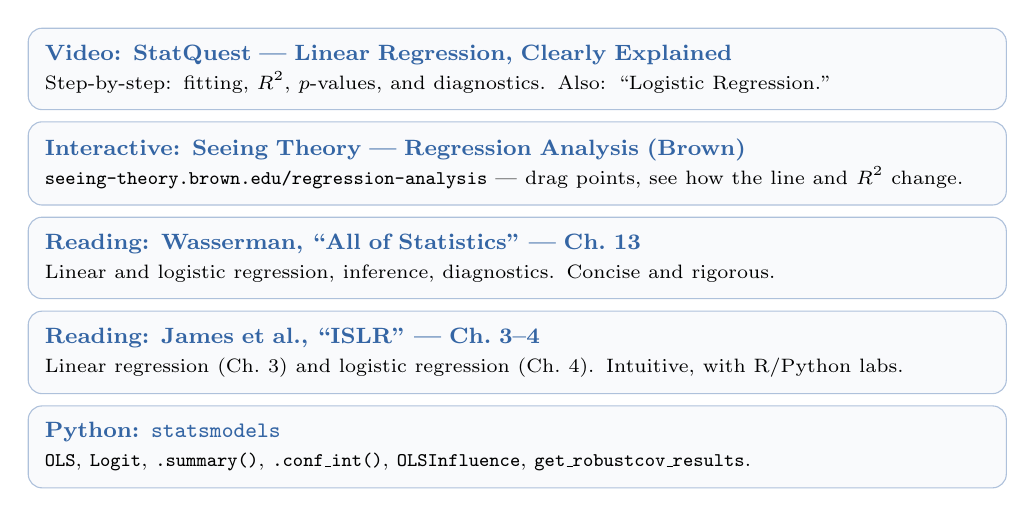
\begin{tikzpicture}[
  rbox/.style={draw=popblue!40, fill=popblue!3, rounded corners=5pt, text width=12cm, align=left, inner sep=6pt, font=\footnotesize}
]
  \node[rbox] at (0, 2.4) {
    \textbf{\textcolor{popblue}{Video: StatQuest --- Linear Regression, Clearly Explained}}\\[1pt]
    \scriptsize Step-by-step: fitting, $R^2$, $p$-values, and diagnostics. Also: ``Logistic Regression.''
  };
  \node[rbox] at (0, 1.2) {
    \textbf{\textcolor{popblue}{Interactive: Seeing Theory --- Regression Analysis (Brown)}}\\[1pt]
    \scriptsize\texttt{seeing-theory.brown.edu/regression-analysis} --- drag points, see how the line and $R^2$ change.
  };
  \node[rbox] at (0, 0.0) {
    \textbf{\textcolor{popblue}{Reading: Wasserman, ``All of Statistics'' --- Ch.\ 13}}\\[1pt]
    \scriptsize Linear and logistic regression, inference, diagnostics. Concise and rigorous.
  };
  \node[rbox] at (0, -1.2) {
    \textbf{\textcolor{popblue}{Reading: James et al., ``ISLR'' --- Ch.\ 3--4}}\\[1pt]
    \scriptsize Linear regression (Ch.\ 3) and logistic regression (Ch.\ 4). Intuitive, with R/Python labs.
  };
  \node[rbox] at (0, -2.4) {
    \textbf{\textcolor{popblue}{Python: \texttt{statsmodels}}}\\[1pt]
    \scriptsize \texttt{OLS}, \texttt{Logit}, \texttt{.summary()}, \texttt{.conf\_int()}, \texttt{OLSInfluence}, \texttt{get\_robustcov\_results}.
  };
\end{tikzpicture}
\end{center}
\end{frame}

\begin{frame}
\begin{center}
  {\Huge\bfseries\textcolor{popblue}{Questions?}}

  \vspace{1cm}

  {\large Next: Lecture~13 --- Generalized linear models}
\end{center}
\end{frame}

\end{document}
